% !TeX spellcheck = en_GB
% !TeX root = ReportMain.tex
\section{Overview of Grading Methods} \label{s:method}
Electric field stress control is important in the design of many power system elements, especially cable terminations and bushings \cite{james2008condition}.
Failure of a bushing can damage the power transformer it is protecting, which can be an expensive mistake \cite{warne2005newnes}.
Bushings are required to withstand Electrical, Mechanical and Thermal stresses as defined in the IEEE standard C57.19.00 \cite{1440990}.
The design of the bushing is largely determined by the insulation material chosen and the resolution of these conflicting sources of stress.
A good bushing design has insulation that can withstand the applied voltage and thermal characteristics appropriate for the current carried by the conductor \cite{harlow2004electric}.

\begin{figure}[!h]
   \centering
   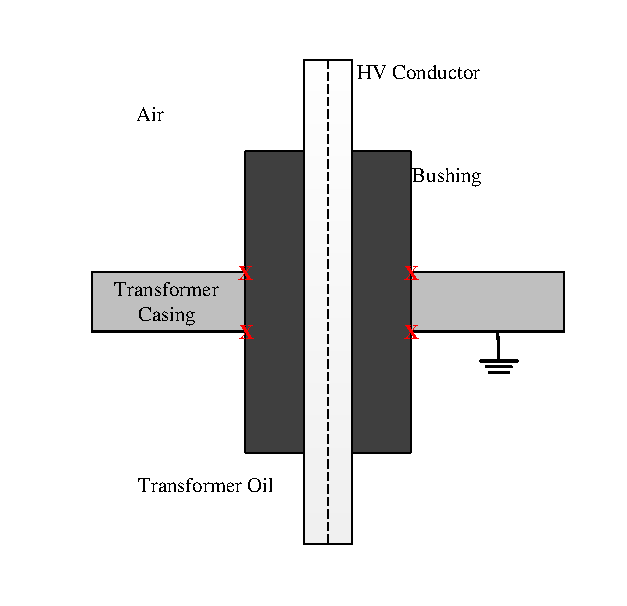
\includegraphics[width = 0.5\textwidth]{GenericBushing.pdf}
   \caption{The Bushing Problem}
   \label{figure:problem}
\end{figure}

The problem grading methods attempt to resolve is laid out in figure \ref{figure:problem}.
The grounded transformer casing is shown in light grey which is perpendicular to the the bushing insulation shown in dark grey and the high voltage conductor in white.
The top of the bushing is exposed to air, while the other side is exposed to transformer oil.
Conducting a numerical analysis or simulation would show that the conductor surface within the plane of the transformer casing and at the points marked by red crosses would experience high electric field stress.
The bushing insulation is designed to withstand the high electric field between the conductor and the transformer casing, however at the points marked with crosses the interface between the solid insulation and the air/transformer oil would cause surface discharge leading to relatively low flashover voltages \cite{kuffel2000high}.
It is therefore necessary to develop methods of reducing electric field stress to a more uniform distribution for both functional purposes and the economic use of space and materials \cite{james2008condition}.

\subsection{Low Voltage and DC Solutions}
There are several methods that can be used dependent upon the application.
Low voltage solutions include internal and external screening electrodes, while resistive stress control can be used for DC applications. Sometimes these solutions are used in combination to achieve an acceptable result.

%%starts here(PPLF)

\subsubsection{External Screening Electrode}

External screening electrodes are parts outside the conductor that are not electrically connected to the conductor. 
They are made of metal conductors such as aluminium. 
Corona ring designs are intended to reduce the electric field strength around the bushing terminal, hence reducing the chance of corona or partial discharge.
Grading ring designs are intended to reduce the potential gradient of insulator, hence reducing the chance of electrical breakdown. 
These screening electrodes come with various shapes according to the different designs. 
The main types of design take the shape of sphere, toroid or ring. 
These are shapes which prevent regions of intense electric field strength by varying the electric potential distribution and help contain electric field as much as possible. 
The reduction in corona discharge not only reduces the power loss, it also suppresses the ageing speed of the insulator. 
An example of these can be seen on figure \ref{Figure:Bush1} and figure \ref{Figure:Bush2}, where they are placed at the top of the bushings. 
The diameters of these designs are closely related to the electric field strength around the electrode, so the diameters of these designs must be carefully considered in order to avoid electrical breakdown.

\subsubsection{Internal Screening Electrode}

Internal screening electrodes are also used to control the electric potential distribution so the electric field strength is within acceptable level to reduce the chance of breakdown. 
They are placed inside the insulator and usually in a pressurised gas. 
Some existing designs have the shape of the internal electrode as a 3D cone and is referred to as a deflector.
There are also designs which are disk shape. 
An example of the field distribution with the cone shape deflector inserted is demonstrated in figure \ref{figure:deflector}.

\begin{figure}[!h]
   \centering
   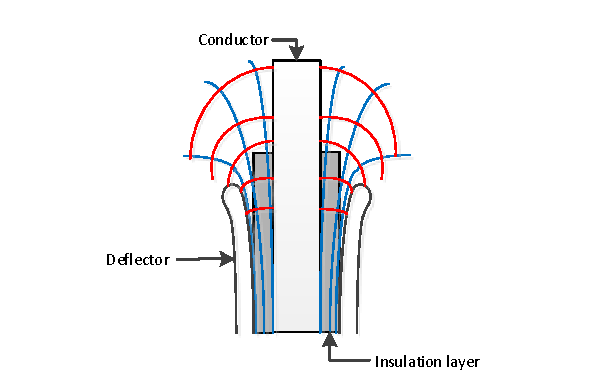
\includegraphics[width = 0.7\textwidth]{Deflector.pdf}
   \caption{Field distribution with deflector}
   \label{figure:deflector}
\end{figure}

\subsection{Capacitive Grading} \label{ss:CapacitiveGrading}
Capacitive grading was first proposed by R.Nagel of Siemens in a German paper published in 1906 \cite{harlow2004electric}.
The value of this type of arrangement was quickly recognised, and is now industry standard practice for AC bushing designs for 25kV - 1500kV applications \cite{james2008condition}.
The general concept of the design is illustrated in figure \ref{figure:fieldgeneric}, showing the isolated foils inserted inside the solid bushing insulation.
Shown in red in figure \ref{figure:fieldgeneric} is the potential field with no grading, and in blue with the isolated conductive foils inserted.
It shows that the whole dielectric is much more evenly stressed with the capacitive grading method.
\begin{figure}[!h]
   \centering
   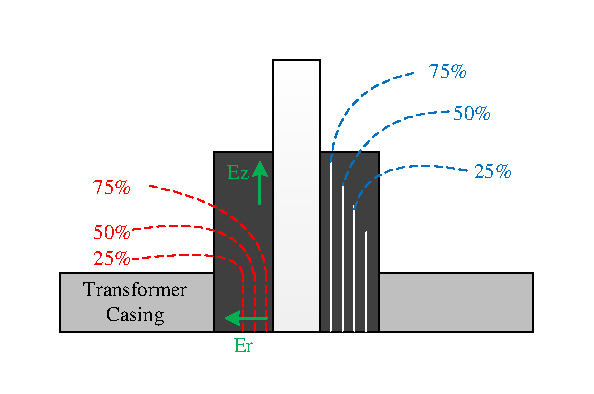
\includegraphics[width = 0.7\textwidth]{BushingFieldDiagram.pdf}
   \caption{Field Distribution both without capacitive grading (shown in red) and with capacitive grading (shown in blue), modified from \cite{james2008condition}}
   \label{figure:fieldgeneric}
\end{figure}

The insulation is stressed in both a radial and axial direction, which sum to give the tangential field.
The radial component $E_r$ can cause breakdown of the insulating material, while the axial component $E_z$ can cause surface discharge along the boundary \cite{Ahmed11}.
Attention must be paid to the design and shape of the boundary, so that the critical value for inception voltage for surface discharge is not exceeded \cite{david2}.
These can be seen in green in figure \ref{figure:fieldgeneric}.
These sum up to give the tangential field $E_t$.

Before proceeding, it is first necessary to introduce some terms.
\begin{figure}[!h]
   \centering
   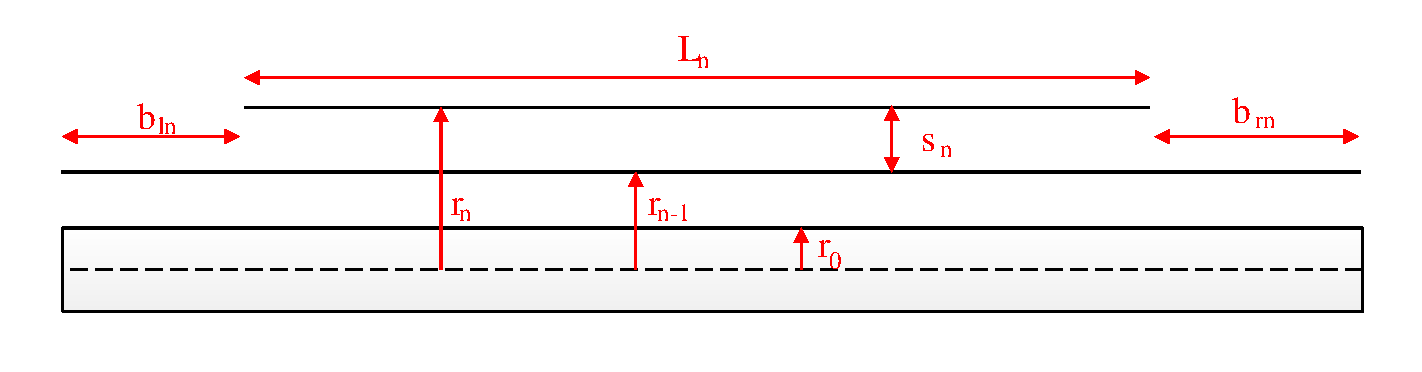
\includegraphics[width = \textwidth]{GradingSymbols.pdf}
   \caption{Symbols for calculating capacitive grading, modified from \cite{Ahmed11}}
   \label{figure:terms}
\end{figure}
Firstly, the radius of the foil is referenced from the centre of the conductor, and termed $r_n$. 
The spacing between each foil is defined in equation \ref{eq:Spacing}.
\begin{equation}
   \label{eq:Spacing}
   S_n = r_n - r_{n-1}
\end{equation}
Additionally, the length of each foil is referred to as $L_n$ and the difference in length on the right and left side between each foil is termed $b_{ln}$ and $b_{rn}$. 
Symmetric double sided capacitive grading is achieved when $b_{ln}=b_{rn}$ \cite{Ahmed11}. 
The total number of foils in the system is $N$.
Also note that subscript $n$ denotes the outermost foil.

Inserting isolated conducting foils forms a set of coaxial capacitor units \cite{kuffel2000high}.
The equation for the capacitance of one of these capacitors depends on the radial displacement $r_n$ and length of each foil $L_n$, as in equation \ref{eq:Cn}.
\begin{equation}
   \label{eq:Cn}
   C_n =\displaystyle\displaystyle\frac{2\pi\epsilon L_{n}}{ln(\displaystyle\frac{r_{n}}{r_{n-1}})}
\end{equation}

The most widely used method to choose the dimensions and locations of the foils is double sided capacitive grading, of which there are two variants; radial grading and axial grading \cite{Ahmed11}.
The aim of capacitive grading is to evenly distribute the electric field between the foils.
To achieve this, an even voltage difference between foils is required as in equation \ref{eq:voltagediff}, where $V$ is the total voltage difference between the conductor and the casing, $N$ is the number of foils required and $\Delta V$ is the voltage between each foil \cite{David1}.
\begin{equation}
   \label{eq:voltagediff}
   \Delta V = \displaystyle\frac{V}{N}
\end{equation}

For the voltage between each foil to be constant, as in equation \ref{eq:voltagediff}, the capacitance between each consecutive pair of foils must also be constant. This is expressed as $C_n = C_{n-1} = \dots = C_0$

\subsubsection{Radial Grading} \label{Section:RadialGrading}
The radial spacing and dimension of each foil is determined in the following derivation, which has been verified and modified from \cite{kuffel2000high}.
In radial grading, the radial component of the electric field $E_r$ is kept constant between all the foils.
The radial electric field is related to the voltage difference and the spacing between each foil, as in equation \ref{eq:radialfield}. $\Delta V$ is already defined as a constant from equation \ref{eq:voltagediff}, and so to have equal field the foil spacing $S_n$ should also be constant. 
\begin{equation}
   \label{eq:radialfield}
   E_r = \displaystyle\displaystyle\frac{\Delta V}{S_n} = Constant
\end{equation}

Given this condition and equation \ref{eq:Cn} for coaxial capacitance, the length of each foil is required to change from foil to foil.
The lengths and radii of consecutive foils can be calculated from the relationship in equation \ref{eq:expcaps}.
%Taking the condition described previous that $C_n = C_{n-1} = \dots = C_0$ and equation \ref{eq:Cn}, equation \ref{eq:expcaps} can be written.
\begin{equation}
   \label{eq:expcaps}
   C_n = \displaystyle\frac{2\pi\epsilon L_{n}}{ln(\displaystyle\frac{r_{n}}{r_{n-1}})} = C_{n-1} = \displaystyle\frac{2\pi\epsilon L_{n-1}}{ln(\displaystyle\frac{r_{n-1}}{r_{n-2}})} = \dots = C_{1} = \displaystyle\frac{2\pi\epsilon L_{1}}{ln(\displaystyle\frac{r_{1}}{r_{0}})}
\end{equation}

The common factor of $2\pi\epsilon$ cancels from equation \ref{eq:expcaps} giving a simple equation linking the lengths and radial displacements of consecutive foils, as in equation \ref{eq:expcaps2}.
\begin{equation}
   \label{eq:expcaps2}
   \displaystyle\frac{L_{n}}{ln(\displaystyle\frac{r_{n}}{r_{n-1}})} = \displaystyle\frac{ L_{n-1}}{ln(\displaystyle\frac{r_{n-1}}{r_{n-2}})} = \dots = \displaystyle\frac{ L_{1}}{ln(\displaystyle\frac{r_{1}}{r_{0}})}
\end{equation}

An approximate solution for thin foils can then be found.
Under the thin foil assumption, $r_{n} = r_{n-1} + S_n$ and $\displaystyle\frac{S_n}{r_n}<<1$ even for the smallest radii of the inner foil.
This is shown in equation \ref{eq:simplefoils}.
%Equation \ref{eq:simplify} allows the simplification of equation \ref{eq:expcaps2} to equation \ref{eq:simplefoils}.

\begin{equation}
   \label{eq:simplify}
   ln(\displaystyle\frac{r_n}{r_{n-1}}) = ln\displaystyle\frac{1}{1-(\displaystyle\frac{S_n}{r_n})} \approx \displaystyle\frac{S_n}{r_n}
\end{equation}

\begin{equation}
   \label{eq:simplefoils}
   L_{n}r_{n} \approx L_{n-1}r_{n-1} \approx \dots \approx L_{1}r_{1}
\end{equation}

Equation \ref{eq:expcaps2} can then be used to determine an exact solution while equation \ref{eq:simplefoils} can be used to find an approximate solution in conjunction with initial data regarding the length and radial displacement of the first foil and the spacing of the foils to calculate the parameters of all the other foils in the bushing. Nevertheless, it should be noted, at this stage, that $r_0$ refers to the surface of the conductor.

\subsubsection{Axial Grading}
In axial grading, the axial component of the electric field $E_z$ is kept constant between all of the foils. 
The following equations prove that the length of each foil must decay by a constant value for each consecutive foil, and the radius at which it is placed is determined by a simple iterative formula.

The axial electric field is related to the voltage difference and the length change between each consecutive foil as in equation \ref{eq:axialfield}. 
Under symmetric capacitive grading, $b_n = b_{ln} = b_{rn}$ with reference to figure \ref{figure:terms}. 
$\Delta V$ is already defined as a constant from equation \ref{eq:voltagediff}, and so to have equal field, the change in foil length $b_n$ should also be constant.
\begin{equation}
   \label{eq:axialfield}
   E_z = \displaystyle\frac{\Delta V}{b_n} = Constant
\end{equation}

The relationship between $L_n$ and $b_n$ is defined in figure \ref{figure:terms}, as explained in equation \ref{eq:length}.
\begin{equation}
   \label{eq:length}
   L_n = L_{n-1} - 2b_n
\end{equation}

Since equation \ref{eq:axialfield} requires the change in foil length $b_n$ to be constant, equation \ref{eq:Cn} for coaxial capacitance requires the radius of each foil to change from foil to foil.
This can be simplified to a similar form as equation \ref{eq:expcaps2}, except that the initial information required, in this case, are different. The necessary parameters are: the length of the first foil($L_1$), the radius of conductor and first foil($r_0,r_1$). However, for initial calculation of $L_n (n=1,2,...N)$ the size of the constant difference in length between each of the foils should be known.All other lengths and radii can then be calculated.

In case of axial grading where different material is used on each side of the bushing ($b_{ln} \neq b_{rn}$) similar calculation is carried out for each side. The total length of each foil is found  by adding $L_{ln}$ and $L_{rn}$. Furthermore, position of each foil could be calculated using the recursive formulae at equation \ref{eq:Axial} 

\begin{equation}
   \label{eq:Axial}
   \displaystyle r_n= \displaystyle  r_{(n-1)} \displaystyle \exp\big( \displaystyle  \frac{L_n}{L_{1}}ln(\displaystyle \frac{r_1}{r_0})\big)
\end{equation}


%\inote{here}

%
%When a conductor is surrounded by concentric foils of dielectric constant $\epsilon$ that is much greater than $\epsilon_{0}$, the system can be treated as a set of coaxial cylindrical capacitor units connected in series.
%In this derivation, the simplest boundary condition is assumed, that is the mean value of the radial field $E_r$ remains constant within the foils.
%The foils are assumed to be of equal thickness, denoted by $\delta$.
%Each of the foils forms a coaxial capacitor stressed by the equal voltage $\Delta V = E_{r}\delta$ providing all capacitances are equal.
%The capacitance of each foil is equal providing $C_n = C_{n-1} = C_0$ where equation \ref{eq:Cn} gives the value of each capacitance.


%This can be expanded as in equation \ref{eq:lengthequals}.
%\begin{equation}
%   \label{eq:lengthequals}
%   \displaystyle\frac{L_n}{ln(\displaystyle\frac{r_{n-1}}{r_{n}})} = \displaystyle\frac{L_{n-1}}{ln(\displaystyle\frac{r_{n-2}}{r_{n-1}})} = \displaystyle\frac{L_1}{ln(\displaystyle\frac{r_{0}}{r_{1}})}
%\end{equation}



%The two methods for solving the recursive equation in equation \ref{eq:simplefoils} is through either radial or axial grading \cite{Ahmed11}.
%In radial grading, the spacing of the foils $S_n$ is assumed to be constant. 
%This means the length of the foils decreases as it it approaches the outer foils of the bushing.
%Equation \ref{eq:evenspace} gives the method to calculate $S_n$ which can then be used in the recursive equation \ref{eq:recursive}, which is a simple form of equation \ref{eq:simplefoils}.
%\begin{equation}
%   \label{eq:evenspace}
%  S_n = \displaystyle\frac{Outer Diameter - Conductor Diameter}{N-1}
%\end{equation}
%
%\begin{equation}
%   \label{eq:recursive}
%  L_{n+1}= L_{n}\displaystyle\frac{r_{n}}{r_{n} + S_{n}}
%\end{equation}


%Radial grading better suits the purposes of this paper, since there is no requirement to assume the length of the final foil.

%\inote{TS - We could derive the recursive equation for axial grading given an assumption of the final foil length here.}